\subsection{RQ3: Changing Bounds}

\begin{figure} 
  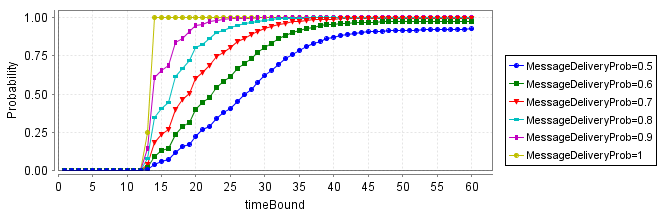
\includegraphics[width=\textwidth]{RQ3-1.png}
  \caption{Probability of Property Satisfied vs Time Bound}
  \label{RQ3-1l}
\end{figure}

For the first set of reading in this experiment we fix the number of retries to 5. The time bound is varied from 1 to 60 steps and probability that the property holds is measured. We repeat this set of reading for different message delivery probabilities. The results are presented in Figure \ref{RQ3-1}, We can clearly see that the time required for inconsistencies to get resolved increases as the probability of message success drops. This supports our hypothesis for the current model. Note that the value at which each curve saturates is slightly different. These are the values that we investigated in RQ2. In fact the MaxRetries = 5 curve in Figure \ref{RQ2-small} follows the saturation values that can be reached for different values of message success probability.